\begin{defn}[Basic Tree]\index{tree}\index{graph!tree}
A \emph{tree} is a \textit{connected} graph with no circuits.
\begin{figure}[H]
    \centering
    %\inputtikz{tree_def}
    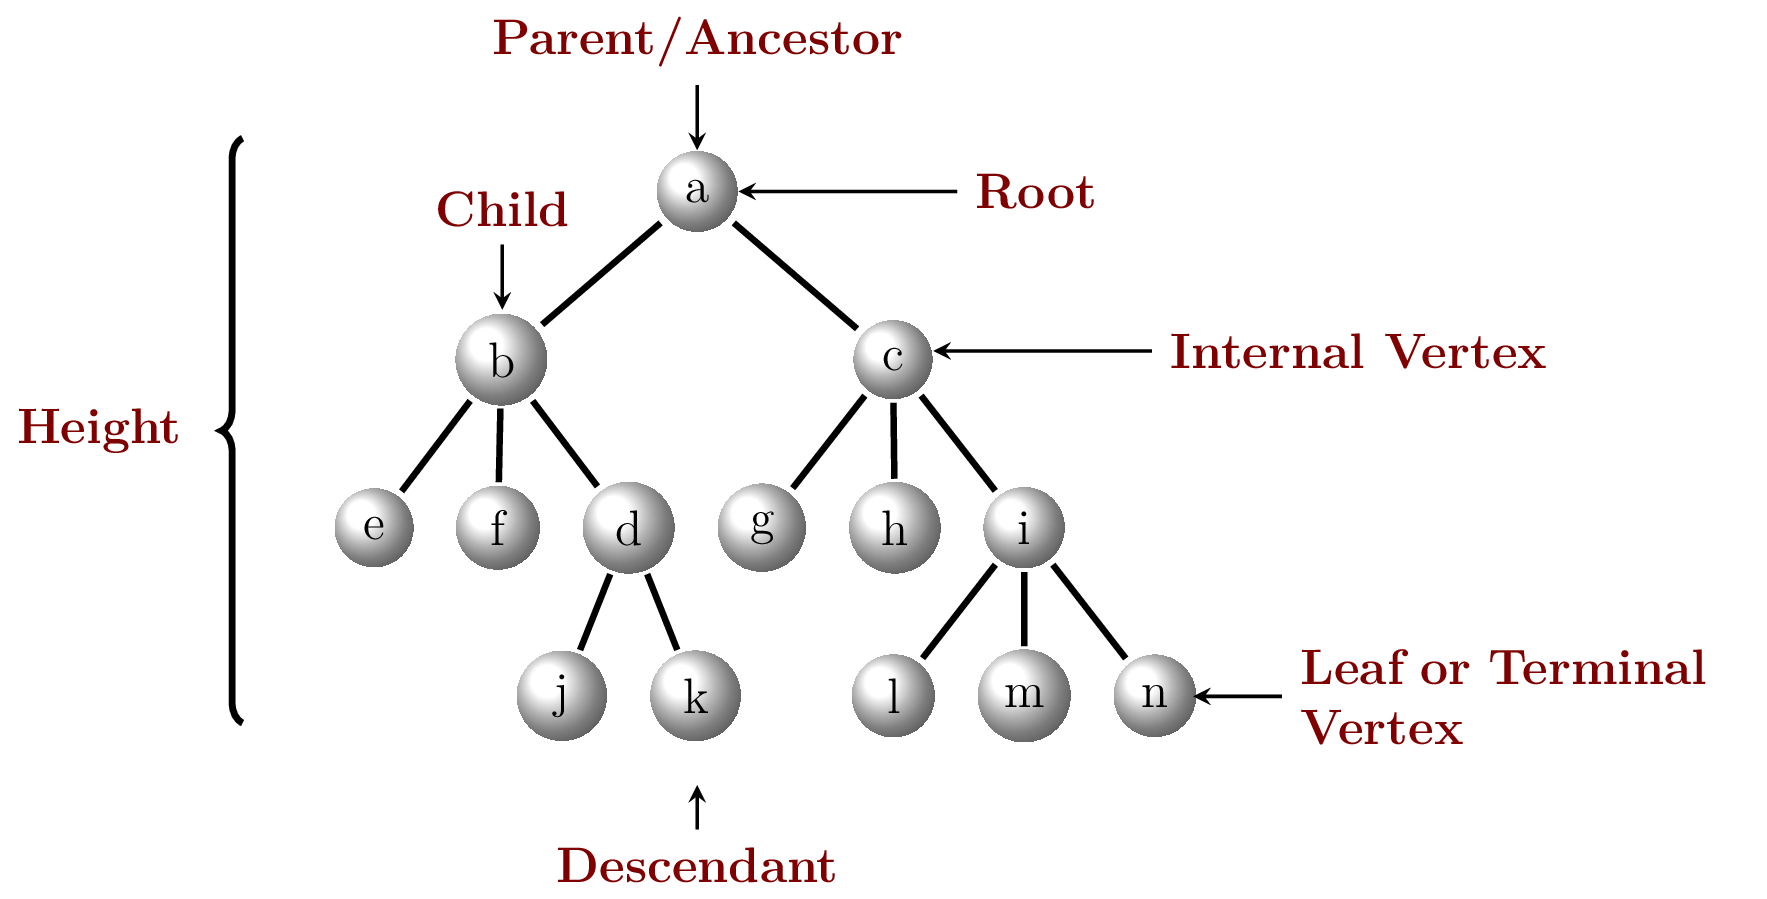
\includegraphics[scale=0.24,alt={image of a tree with lables for different components}]{images/created/tree_def.png}
    \caption{Basic Tree Terminology}
    \label{fig:tree_terms}
\end{figure}
\end{defn}

\begin{thm}
    Every tree has a vertex of degree 1.
\end{thm}

\begin{thm}
    A tree with \(n\) vertices has \(n-1\) edges.
\end{thm}

\begin{defn}[Binary Trees]\index{binary trees}\index{tree!binary}\index{full binary tree}\index{tree!full binary}
\hspace*{1in}
\begin{itemize}
    \item A \emph{binary tree} is a tree in which each parent has \hrulefill .
    \item A \emph{full binary tree} is a tree in which each parent has \hrulefill .
\end{itemize}
\begin{figure}[H]
    \centering
    %\inputtikz{trees_binary}
    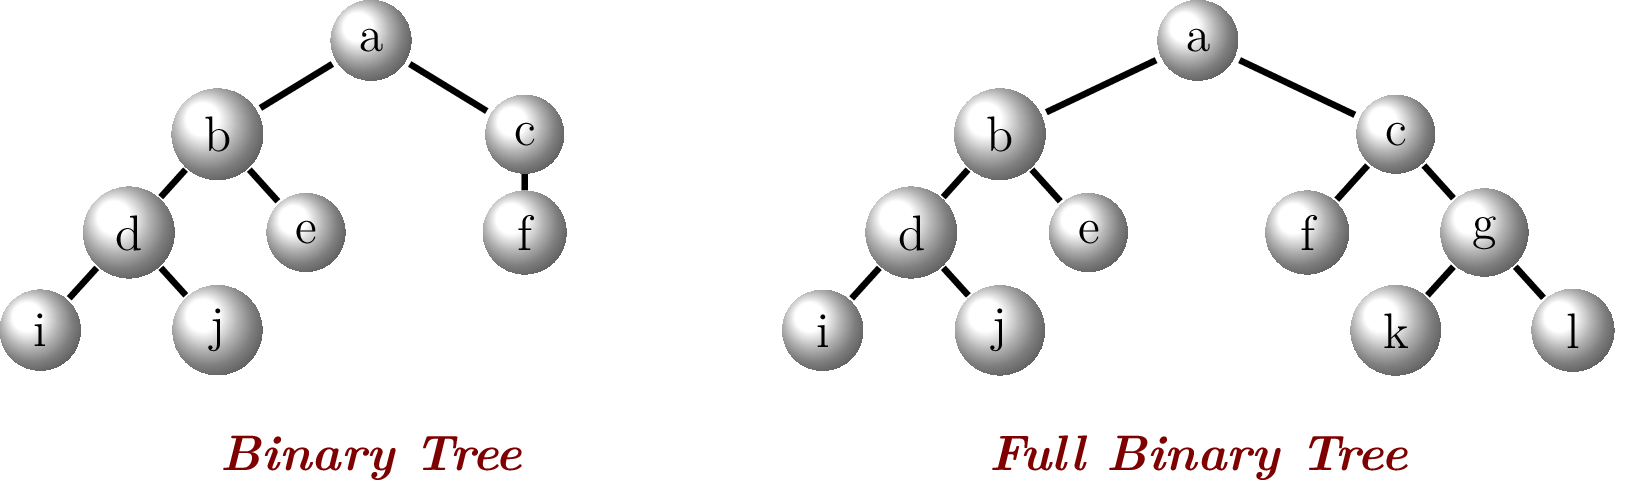
\includegraphics[scale=0.24,alt={basic binary tree}]{images/created/trees_binary.png}
    \caption{Types of Binary Trees}
    \label{fig:binary_trees}
\end{figure}
\end{defn}

\clearpage

\begin{thm}
    Given a full binary tree with \(k\) internal vertices, there are \(n=2k+1\) vertices all together and so \(k+1\) leaves.
    \begin{figure}[H]
        \centering
        %\inputtikz{tree_full_binary}
	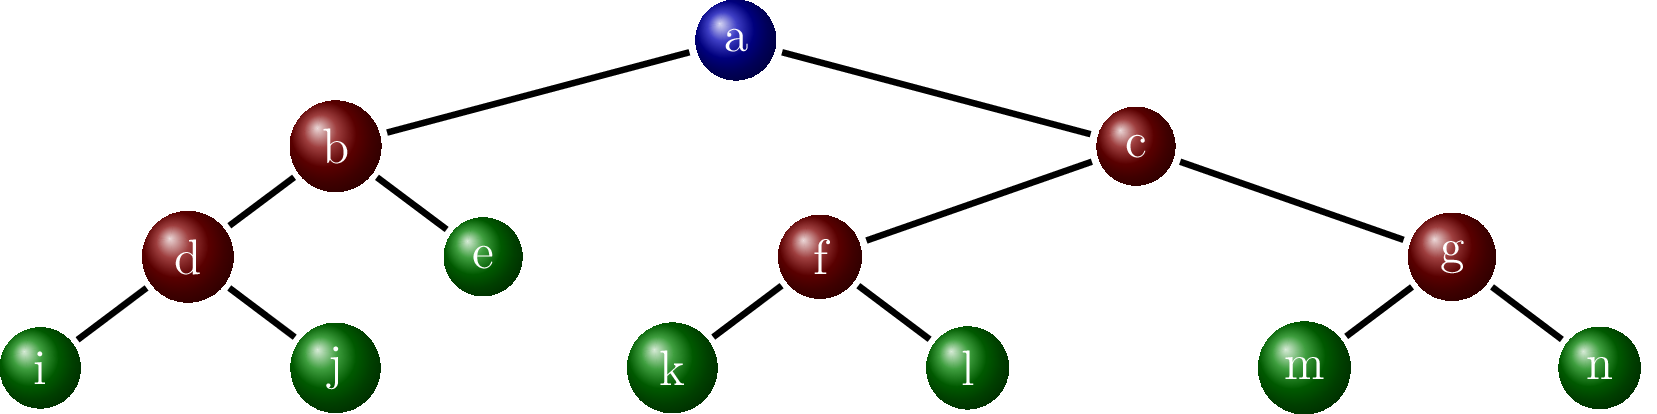
\includegraphics[scale=0.24,alt={full binary tree}]{images/created/tree_full_binary.png}
        \caption{Vertices in a Full Binary Tree}
        \label{fig:full_tree}
    \end{figure}
\end{thm}

\begin{thm}
    Given a binary tree of height \(h\) with \(t\) leaves, \emph{\(t\leq 2^h\)} or equivalently \emph{\(\log_2(t)\leq h\)}.
    Equality occurs in full binary trees in which all leaves are the same height.
\end{thm}

\begin{practiceprob}
Label each of the following as true for false and include reasons:
\begin{enumerate}
    \setlength\itemsep{3\baselineskip}
    \item The total degree of a tree is equal to \(2n-2\) for some \(n\).
    \item There exists a connected graph with 7 vertices and 7 edges.
    \item There exists a tree with 7 vertices and 7 edges.
    \item There exists a tree with 7 vertices and 6 edges.
    \item A graph with 7 vertices and 6 edges is a tree.
    \item A connected graph with 10 vertices and total degree 18 is a tree.\vspace{3\baselineskip}
\end{enumerate}
\end{practiceprob}